\section{Reakcja na losowe wejście}
\label{sec:losowe-wejscie}

Rozdział opisuje, do jakich stanów dochodzi nauczona sieć, gdy na wejście poda się losowy stan zamiast uszkodzonego wzorca. Wykorzystano eksperymenty \texttt{random} i \texttt{random-load} z Tabeli~\ref{tab:eksperymenty}. W każdej komórce sieć dostaje \num{10000} losowych wejść (rozdział~\ref{sec:uszkodzenia}), tych samych dla obu reguł i obu trybów.

\subsection{Stany końcowe}
\label{sec:losowe-klasy}

Klasy stanów końcowych pokazano na Rysunku~\ref{fig:losowe-klasy}. Przy regule Oji losowe wejście kończy we wzorcu albo w jego negacji w około połowie przypadków lub częściej, poza \texttt{letters-14x20}. Przy regule Hebba w sześciu z ośmiu zbiorów ponad \qty{90}{\percent} wejść kończy w stanie pozornym. Reguła Hebba może doprowadzić tylko do wzorców stabilnych (rozdział~\ref{sec:stabilnosc}), więc w zbiorach liter i w \texttt{large-25x50} nie osiąga żadnego wzorca. Wzorzec i jego negacja są osiągane równie często, bo $E(-s) = E(s)$, a losowe wejście jest symetryczne względem negacji (rozdział~\ref{sec:stany-pozorne}). Cykle długości 2 występują tylko w trybie synchronicznym, zgodnie z rozdziałem~\ref{sec:model}, a żaden przebieg nie osiągnął limitu kroków.

\begin{figure}[H]
    \centering
    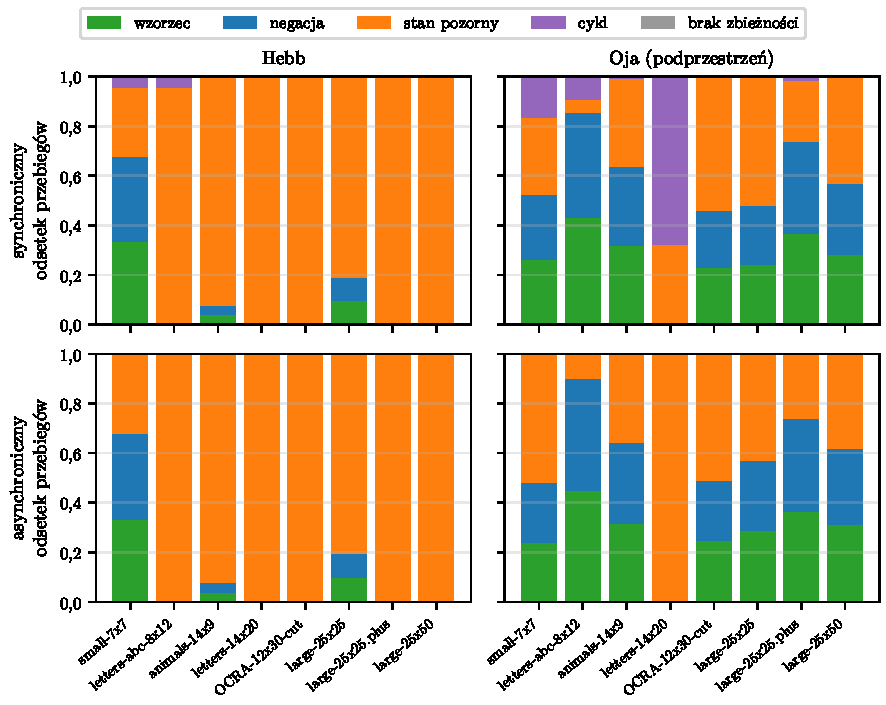
\includegraphics[width=0.8\textwidth]{random/figures/outcomes.pdf}
    \caption{Klasy stanów końcowych dla \num{10000} losowych wejść na komórkę. Górne wykresy: tryb synchroniczny. Dolne wykresy: tryb asynchroniczny. Lewa kolumna: reguła Hebba. Prawa kolumna: reguła Oji.}
    \label{fig:losowe-klasy}
\end{figure}

\noindent Reguły różnią się też liczbą stanów pozornych. Przy regule Hebba jest ich od 2 do 14, z wyjątkiem \texttt{large-25x25} (209 w trybie synchronicznym i 142 w asynchronicznym), a każdy przyciąga dużą część wejść. W \texttt{letters-abc-8x12}, \texttt{letters-14x20} i \texttt{large-25x25.plus} jeden stan pozorny i jego negacja zbierają po około połowie wszystkich wejść. Przy regule Oji stanów pozornych jest od 2 w \texttt{letters-abc-8x12} do kilku tysięcy, a najczęstszy z nich zbiera około \num{0.05} wejść. Wyjątkiem jest \texttt{letters-14x20}, w którym wejścia prawie nigdy nie trafiają do wzorca, a w trybie asynchronicznym kończą w \num{9399} różnych stanach pozornych na \num{10000} wejść.

Reguła Oji daje wszystkim wzorcom podobną szansę. Stosunek odsetka wejść kończących w najczęściej i najrzadziej osiąganym wzorcu (razem z negacją) wynosi od \num{1.08} do \num{2.44}, poza \texttt{letters-14x20}. Przy regule Hebba osiągane wzorce są bardzo nierówno dostępne, na przykład w \texttt{small-7x7} od \num{0.022} do \num{0.600} wejść, co opisali już Hopfield, Feinstein i Palmer~\cite{hopfield1983}.

\subsection{Stany pozorne i energia}
\label{sec:losowe-energia}

Energie stanów końcowych, pokazane na Rysunku~\ref{fig:losowe-energie}, wyjaśniają różnicę między regułami. Przy regule Oji każdy osiągnięty wzorzec ma tę samą energię $-(N - p)/2$, na przykład $\num{-309.5}$ w \texttt{large-25x25}, poza \texttt{letters-14x20}, w którym wynosi ona $\num{-127.505}$ zamiast $\num{-127}$. Żaden stan pozorny w żadnym zbiorze nie ma energii niższej. Zgadza się to z~\eqref{eq:energia-rzut}: wzorce leżą w podprzestrzeni wzorców, więc są minimami globalnymi energii. Przy regule Hebba najniższą energię mają stany pozorne. W \texttt{large-25x25.plus} dominujący stan pozorny ma energię $\num{-965.4}$, a jedyny osiągany wzorzec $\num{-327.2}$. Wejścia kończą w stanie pozornym niższym od każdego osiąganego wzorca w \num{0.92} przypadków w \texttt{animals-14x9}, \num{0.996} w \texttt{OCRA-12x30-cut} i \num{0.997} w \texttt{large-25x25.plus}. Wyjątkiem jest \texttt{small-7x7}, w którym najniżej leży jeden ze wzorców. Głębokie minima energii mają też duże obszary przyciągania~\cite{hopfield1983}, dlatego losowe wejście najczęściej do nich trafia.

\begin{figure}[H]
    \centering
    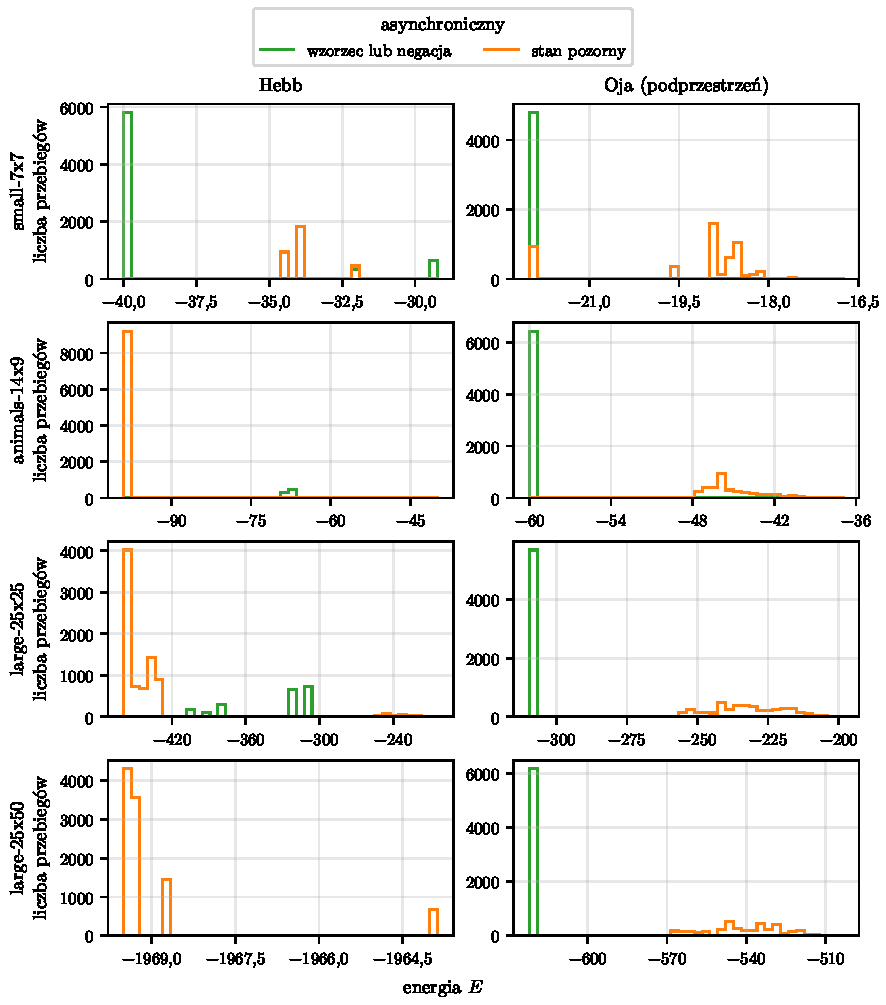
\includegraphics[width=0.7\textwidth]{random/figures/energies.pdf}
    \caption{Histogramy energii stanów końcowych dla \num{10000} losowych wejść w czterech zbiorach (tryb asynchroniczny). Lewa kolumna: reguła Hebba. Prawa kolumna: reguła Oji.}
    \label{fig:losowe-energie}
\end{figure}

\noindent Typowy głęboki stan pozorny reguły Hebba pokazano na Rysunku~\ref{fig:losowe-przebieg}. To samo losowe wejście zbioru \texttt{letters-abc-8x12} przy regule Hebba kończy w stanie $\operatorname{sgn}(\xi^0 + \xi^1 + \xi^2)$, czyli w mieszaninie trzech liter z rozdziału~\ref{sec:stany-pozorne}, a przy regule Oji w literze a. W tym zbiorze przy regule Hebba w takiej mieszaninie albo w jej negacji kończą wszystkie wejścia w trybie asynchronicznym i \num{0.956} wejść w synchronicznym (reszta to cykle). W \texttt{large-25x50} i \texttt{OCRA-12x30-cut} część wejść kończy w mieszaninach pięciu wzorców.

\begin{figure}[H]
    \centering
    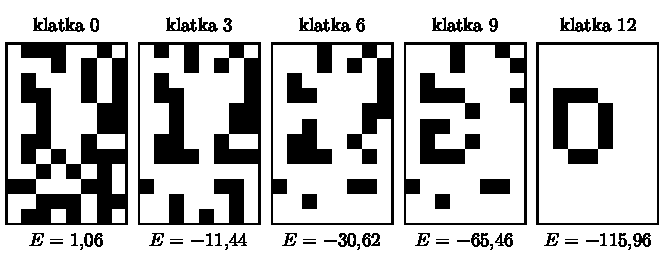
\includegraphics[width=0.75\textwidth]{random/figures/recall-random-hebb.pdf}

    \vspace{0.2cm}
    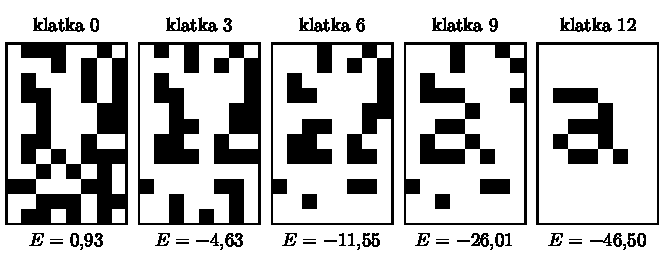
\includegraphics[width=0.75\textwidth]{random/figures/recall-random-oja.pdf}
    \caption{Odtwarzanie z tego samego losowego wejścia w zbiorze \texttt{letters-abc-8x12} (tryb asynchroniczny, klatka co 8 aktualizacji). Górny wykres: reguła Hebba, stan końcowy to mieszanina trzech liter. Dolny wykres: reguła Oji, stan końcowy to litera a.}
    \label{fig:losowe-przebieg}
\end{figure}

\subsection{Liczba wzorców}
\label{sec:losowe-licznosc}

Wpływ liczby wzorców na reakcję na losowe wejście pokazano na Rysunku~\ref{fig:losowe-licznosc} dla początkowych fragmentów zbiorów \texttt{large-25x25.plus} i \texttt{letters-14x20}. Przy trzech obrazach obie reguły mają po 8 stanów pozornych i wszystkie są mieszaninami trzech wzorców (cztery kombinacje znaków i ich negacje). Przy regule Hebba z każdym kolejnym wzorcem coraz mniej wejść trafia do wzorców (z \num{0.71} przy $p = 3$ do \num{0.003} przy $p = 15$), bo wzorce tracą stabilność, a kilka głębokich stanów pozornych zbiera prawie wszystkie wejścia. Przy regule Oji odsetek wejść kończących we wzorcu dla obrazów nie spada i wynosi od \num{0.48} do \num{0.74}. Dla liter od $p = 15$ wejścia prawie nigdy nie trafiają do wzorca: w trybie synchronicznym ponad \num{0.6} z nich kończy w cyklu, a w asynchronicznym w tysiącach różnych stanów pozornych.

\begin{figure}[H]
    \centering
    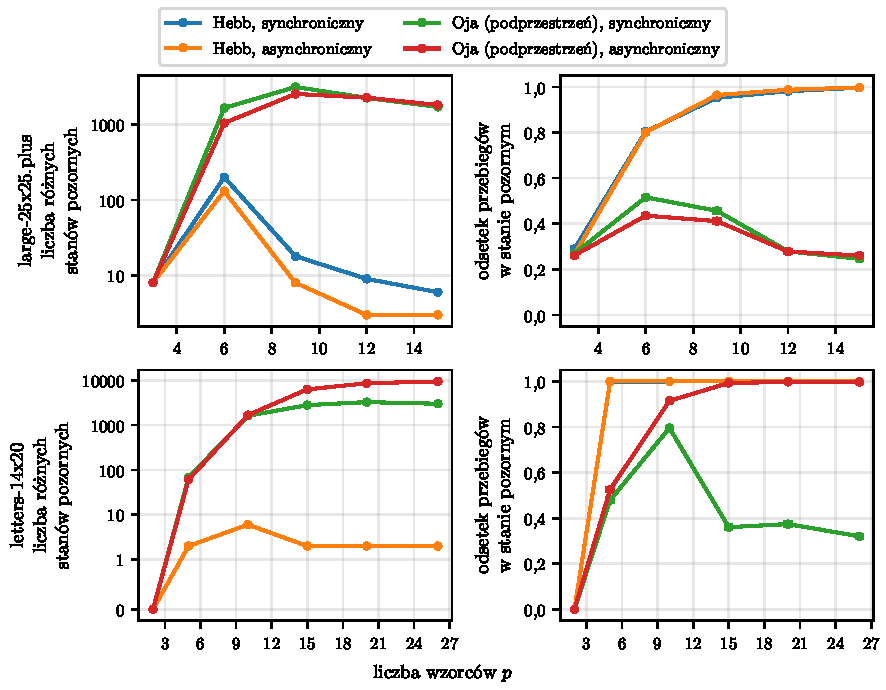
\includegraphics[width=0.62\textwidth]{random-load/figures/distinct.pdf}
    \caption{Liczba różnych stanów pozornych (lewa kolumna) i odsetek wejść kończących w stanie pozornym (prawa kolumna) w zależności od liczby wzorców $p$ dla początkowych fragmentów zbiorów \texttt{large-25x25.plus} (górne wykresy) i \texttt{letters-14x20} (dolne wykresy).}
    \label{fig:losowe-licznosc}
\end{figure}
